\section{Material Models and Results}
\label{sec:bayesian:results}

We now demonstrate the effectiveness of our technique by fitting several procedural material models to a mix of synthetic and real target images.

Our forward evaluation process uses collocated camera and light.
This configuration closely matches a mobile phone camera with flash (which is used for most of the real target images) and simplifies some BRDF formulations (because the incoming, outgoing, and half-way vectors are all identical).
Further, we assume that the distance between camera and sample is known as it is generally easy to measure or estimate.
The knowledge of the camera field of view allows us to compute the physical scale of the resulting pixels.
Lastly, we treat light intensity and camera vignetting (expressed as an image-space Gaussian function) as (unknown) parameters of the forward evaluation process so that they do not need to be calibrated.
Our parameter inference framework presented in \S\ref{sec:bayesian:summary} and \S\ref{sec:bayesian:param} is not limited to this specific setup.

All the procedural material models we used, which will be detailed in \S\ref{ssec:proc_models}, are implemented using \textsf{PyTorch} which automatically provides GPU acceleration and computes derivatives through backpropagation. 
For all material parameter inference tasks, our forward evaluation generates $512 \times 512$ images.
Notice that the recovered parameters can then be used to generate results with much higher resolution because the procedural models are generally resolution-independent.

\subsection{Similarity Relations in Translucency}

As a motivating example, we first illustrate the behavior of the MCMC material parameter estimation process on the case of a homogeneous translucent material with two varying parameters.
In this example, the shape of the posterior can be analytically derived (using the similarity theory) and easily plotted. This serves as a demonstration and validation of our approach.

\begin{figure}[h]
	\centering
	\begin{tabular}{c}
		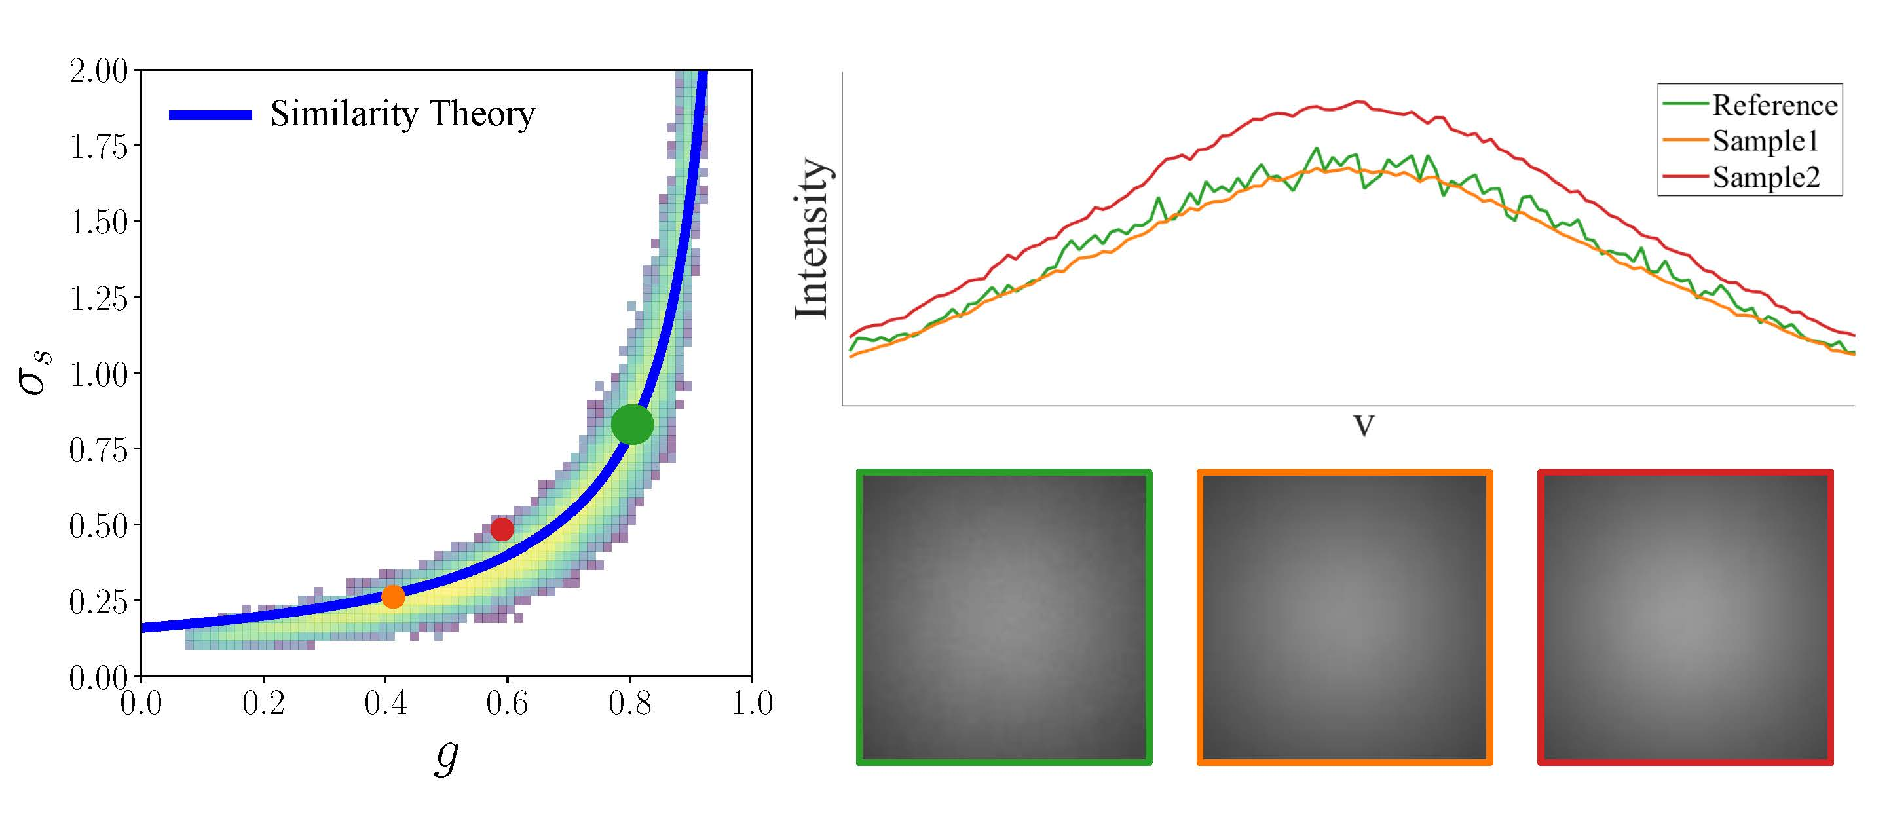
\includegraphics[width=0.98\columnwidth]{bayesian/fig4/scatter.pdf}
	\end{tabular}
	\caption[]{\label{fig:bayesian:scatter}
		A motivating example of a scattering material with two estimated parameters (scattering coefficient and phase function parameter). The posterior distribution sampled with our method for three synthetic input images is able to detect the full structure of the parameter space, matching the predictions from similarity theory.
	}
\end{figure}


Specifically, the material parameter space of translucent materials under the radiative transfer framework \cite{chandrasekhar1960radiative} is known to be approximately over-complete~\cite{zhao2014high}.
Specifically, two sets of parameters $(\sigma_s, \sigma_a, g)$ and $(\sigma_s^*, \sigma_a^*, g^*)$ satisfying the following \emph{similarity relation} usually yield similar final appearances:
\begin{equation}
	\label{eq:similarity_rel}
	\sigma_a = \sigma_a^*, \quad (1 - g)\,\sigma_s = (1 - g^*)\,\sigma_s^*,
\end{equation}
where $\sigma_a$ and $\sigma_s$ are, respectively, the absorption and scattering coefficients, and $g$ is the first Legendre moment of the phase function.
We show in Figure~\ref{fig:bayesian:scatter} that applying our Bayesian inference method to $\sigma_s$ and $g$ (with fixed $\sigma_a$) computes a posterior distribution that agrees well with the predicted similarity relation~\eqref{eq:similarity_rel}.


\subsection{Procedural Material Models}
\label{ssec:proc_models}

We show results generated using synthetic images in Figures \ref{fig:bayesian:synthetic} and \ref{fig:bayesian:discrete} as well as real photographs (taken with different cameras) in Figure \ref{fig:bayesian:real}.
Please see the supplemental material for more results, including animations illustrating point estimations and sampling. Below we describe the six procedural models tested. Please refer to the supplement for additional detail and a \textsf{PyTorch} implementation. For each parameter, we define a reasonable truncated Gaussian distribution as its prior (also see supplement). In most cases, the MCMC sampling starts from the peak of the prior. In some examples (e.g wood), we first run posterior maximization and then switch to sampling from the optimized point. We drop some number (typically 200 to 1000) of initial MCMC samples due to burn-in.

\begin{table}[h]
	\centering
	\caption[Performance]{\label{tab:bayesian:performance}
		Performance statistics for our MCMC-based posterior sampling.
		The numbers are collected using a workstation equipped with an Intel i7-6800K six-core CPU and an Nvidia GTX 1080 GPU.
	}
	\addtolength{\tabcolsep}{3pt}
	\begin{tabular}{c|cccccc}
		Material & bump & leather & plaster & flakes & metal & wood\\
		\hline
		\# of parameters. & 8 & 12 & 11 & 13 & 10 & 23\\
		MCMC (1k iter.) & 180s & 194s & 190s & 187s & 182s & 290s
	\end{tabular}
\end{table}


\renewcommand{\imglabel}[1]{\put(2,5){\tiny\contour{black}{\textcolor{white}{\textbf{#1}}}}}
\begin{figure}[!ht]
	\centering
	\setlength{\resLen}{0.12\columnwidth}	
	\addtolength{\tabcolsep}{-5pt}
	\begin{tabular}{ccccccccc}
		Target & S1 & S2 & S3 & & Target & S1 & S2 & S3
		\\
		\begin{overpic}[width=\resLen]{bayesian/fig5/1_bump_1/target.jpg}
			\imglabel{Bump-1}
		\end{overpic} &
		\includegraphics[width=\resLen]{bayesian/fig5/1_bump_1/good1.jpg} &
		\includegraphics[width=\resLen]{bayesian/fig5/1_bump_1/good2.jpg} &
		\includegraphics[width=\resLen]{bayesian/fig5/1_bump_1/bad1.jpg} &
		&
		\begin{overpic}[width=\resLen]{bayesian/fig5/1_bump_2/target.jpg}
			\imglabel{Bump-2}
		\end{overpic} &
		\includegraphics[width=\resLen]{bayesian/fig5/1_bump_2/good1.jpg} &
		\includegraphics[width=\resLen]{bayesian/fig5/1_bump_2/good2.jpg} &
		\includegraphics[width=\resLen]{bayesian/fig5/1_bump_2/bad1.jpg}
		\\
		\begin{overpic}[width=\resLen]{bayesian/fig5/2_leather_1/target.jpg}
			\imglabel{Leather-1}
		\end{overpic} &
		\includegraphics[width=\resLen]{bayesian/fig5/2_leather_1/good1.jpg} &
		\includegraphics[width=\resLen]{bayesian/fig5/2_leather_1/good2.jpg} &
		\includegraphics[width=\resLen]{bayesian/fig5/2_leather_1/bad1.jpg} &
		&
		\begin{overpic}[width=\resLen]{bayesian/fig5/2_leather_2/target.jpg}
			\imglabel{Leather-2}
		\end{overpic} &
		\includegraphics[width=\resLen]{bayesian/fig5/2_leather_2/good1.jpg} &
		\includegraphics[width=\resLen]{bayesian/fig5/2_leather_2/good2.jpg} &
		\includegraphics[width=\resLen]{bayesian/fig5/2_leather_2/bad1.jpg}
		\\
		\begin{overpic}[width=\resLen]{bayesian/fig5/3_plaster_1/target.jpg}
			\imglabel{Plaster-1}
		\end{overpic} &
		\includegraphics[width=\resLen]{bayesian/fig5/3_plaster_1/good1.jpg} &
		\includegraphics[width=\resLen]{bayesian/fig5/3_plaster_1/good2.jpg} &
		\includegraphics[width=\resLen]{bayesian/fig5/3_plaster_1/bad1.jpg} &
		&
		\begin{overpic}[width=\resLen]{bayesian/fig5/3_plaster_2/target.jpg}
			\imglabel{Plaster-2}
		\end{overpic} &
		\includegraphics[width=\resLen]{bayesian/fig5/3_plaster_2/good1.jpg} &
		\includegraphics[width=\resLen]{bayesian/fig5/3_plaster_2/good2.jpg} &
		\includegraphics[width=\resLen]{bayesian/fig5/3_plaster_2/bad1.jpg}
		\\
		\begin{overpic}[width=\resLen]{bayesian/fig5/4_flake_1/target.jpg}
			\imglabel{Metallicflake-1}
		\end{overpic} &
		\includegraphics[width=\resLen]{bayesian/fig5/4_flake_1/good1.jpg} &
		\includegraphics[width=\resLen]{bayesian/fig5/4_flake_1/good2.jpg} &
		\includegraphics[width=\resLen]{bayesian/fig5/4_flake_1/bad1.jpg} &
		&
		\begin{overpic}[width=\resLen]{bayesian/fig5/4_flake_2/target.jpg}
			\imglabel{Metallicflake-2}
		\end{overpic} &
		\includegraphics[width=\resLen]{bayesian/fig5/4_flake_2/good1.jpg} &
		\includegraphics[width=\resLen]{bayesian/fig5/4_flake_2/good2.jpg} &
		\includegraphics[width=\resLen]{bayesian/fig5/4_flake_2/bad1.jpg}
		\\
		\begin{overpic}[width=\resLen]{bayesian/fig5/5_metal_1/target.jpg}
			\imglabel{Brushmetal-1}
		\end{overpic} &
		\includegraphics[width=\resLen]{bayesian/fig5/5_metal_1/good1.jpg} &
		\includegraphics[width=\resLen]{bayesian/fig5/5_metal_1/good2.jpg} &
		\includegraphics[width=\resLen]{bayesian/fig5/5_metal_1/bad1.jpg} &
		&
		\begin{overpic}[width=\resLen]{bayesian/fig5/5_metal_2/target.jpg}
			\imglabel{Brushmetal-2}
		\end{overpic} &
		\includegraphics[width=\resLen]{bayesian/fig5/5_metal_2/good1.jpg} &
		\includegraphics[width=\resLen]{bayesian/fig5/5_metal_2/good2.jpg} &
		\includegraphics[width=\resLen]{bayesian/fig5/5_metal_2/bad1.jpg}
		\\
		\begin{overpic}[width=\resLen]{bayesian/fig5/6_wood_1/target.jpg}
			\imglabel{Wood-1}
		\end{overpic} &
		\includegraphics[width=\resLen]{bayesian/fig5/6_wood_1/good1.jpg} &
		\includegraphics[width=\resLen]{bayesian/fig5/6_wood_1/good2.jpg} &
		\includegraphics[width=\resLen]{bayesian/fig5/6_wood_1/bad1.jpg} & &
		\begin{overpic}[width=\resLen]{bayesian/fig5/6_wood_2/target.jpg}
			\imglabel{Wood-2}
		\end{overpic} &
		\includegraphics[width=\resLen]{bayesian/fig5/6_wood_2/good1.jpg} &
		\includegraphics[width=\resLen]{bayesian/fig5/6_wood_2/good2.jpg} &
		\includegraphics[width=\resLen]{bayesian/fig5/6_wood_2/bad1.jpg}
	\end{tabular}
	\caption[Synthetic results]{\label{fig:bayesian:synthetic}
		\textbf{Results} of our MCMC sampling on \textbf{synthetic} inputs. Each row corresponds to two examples of a different material model. For each example, the first column is the synthetic target image. We show MCMC samples in the other columns, where S1 and S2 are chosen closer to the peak of the posterior distribution, and S3 is further away. More results please refer to supplemental materials.
	}
\end{figure}


\renewcommand{\imglabel}[1]{\put(2,5){\scriptsize\contour{black}{\textcolor{white}{\textbf{#1}}}}}
\begin{figure}[!ht]
	\centering
	\setlength{\resLen}{0.12\columnwidth}	
	\addtolength{\tabcolsep}{-5pt}
	\begin{tabular}{cccccccc}
		Target & S1 & S2 & S3 & Target & S1 & S2 & S3
		\\
		\begin{overpic}[width=\resLen]{bayesian/fig6/2_leather_1/target.jpg}
			\imglabel{Leather-1}
		\end{overpic} &
		\includegraphics[width=\resLen]{bayesian/fig6/2_leather_1/good1.jpg} &
		\includegraphics[width=\resLen]{bayesian/fig6/2_leather_1/bad1.jpg} &
		\includegraphics[width=\resLen]{bayesian/fig6/2_leather_1/bad2.jpg} &
		\begin{overpic}[width=\resLen]{bayesian/fig6/3_plaster_2/target.jpg}
			\imglabel{Plaster-2}
		\end{overpic} &
		\includegraphics[width=\resLen]{bayesian/fig6/3_plaster_2/good1.jpg} &
		\includegraphics[width=\resLen]{bayesian/fig6/3_plaster_2/bad1.jpg} &
		\includegraphics[width=\resLen]{bayesian/fig6/3_plaster_2/bad2.jpg}
		\\
		&
		\begin{overpic}[width=\resLen]{bayesian/fig6/cell/cell_1.jpg}
			\put(0,0){\color{green}%
				\frame{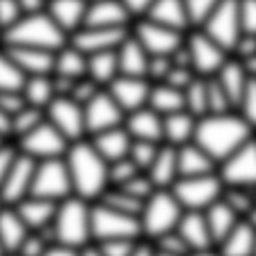
\includegraphics[width=0.4\resLen]{bayesian/fig6/cell/cell_1_zoom.jpg}}}
		\end{overpic}
		&
		\begin{overpic}[width=\resLen]{bayesian/fig6/cell/cell_2.jpg}
			\put(0,0){\color{green}%
				\frame{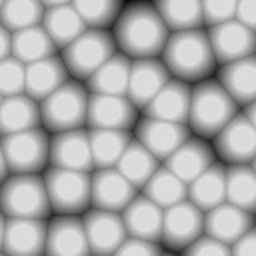
\includegraphics[width=0.4\resLen]{bayesian/fig6/cell/cell_2_zoom.jpg}}}
		\end{overpic}
		&
		\begin{overpic}[width=\resLen]{bayesian/fig6/cell/cell_3.jpg}
			\put(0,0){\color{green}%
				\frame{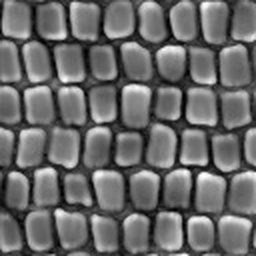
\includegraphics[width=0.4\resLen]{bayesian/fig6/cell/cell_3_zoom.jpg}}}
		\end{overpic}
		&
		&
		\begin{overpic}[width=\resLen]{bayesian/fig6/noise/noise_1.jpg}
			\put(0,0){\color{green}%
				\frame{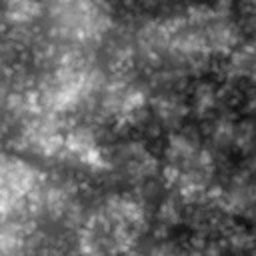
\includegraphics[width=0.4\resLen]{bayesian/fig6/noise/noise_1_zoom.jpg}}}
		\end{overpic}
		&
		\begin{overpic}[width=\resLen]{bayesian/fig6/noise/noise_2.jpg}
			\put(0,0){\color{green}%
				\frame{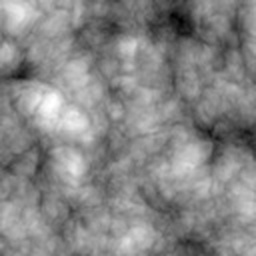
\includegraphics[width=0.4\resLen]{bayesian/fig6/noise/noise_2_zoom.jpg}}}
		\end{overpic}
		&
		\begin{overpic}[width=\resLen]{bayesian/fig6/noise/noise_3.jpg}
			\put(0,0){\color{green}%
				\frame{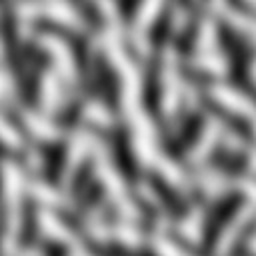
\includegraphics[width=0.4\resLen]{bayesian/fig6/noise/noise_3_zoom.jpg}}}
		\end{overpic}
	\end{tabular}
	\caption[Synthetic results with discrete parameters]{\label{fig:bayesian:discrete}
		\textbf{MCMC sampling with discrete parameters.} In these examples, we illustrate the ability of our sampling to handle discrete parameters. In both examples, one noise inputs used in the procedural model can be switched between several different types of noise. Out of the thousands of sampled solutions, we pick three that have different settings of the discrete parameter where the (log) pdf values decrease from S1 to S3.
	}
\end{figure}


\renewcommand{\imglabel}[1]{\put(2,5){\tiny\contour{black}{\textcolor{white}{\textbf{#1}}}}}
\begin{figure}[h!]
	\centering
	\setlength{\resLen}{0.12\columnwidth}	
	\addtolength{\tabcolsep}{-5pt}
	\begin{tabular}{ccccccccc}
		Photo & S1 & S2 & S3 & & Photo & S1 & S2 & S3
		\\
		\begin{overpic}[width=\resLen]{bayesian/fig7/1_bump_3/target.jpg}
			\imglabel{Bump-3}
		\end{overpic} &
		\includegraphics[width=\resLen]{bayesian/fig7/1_bump_3/good1.jpg} &
		\includegraphics[width=\resLen]{bayesian/fig7/1_bump_3/good2.jpg} &
		\includegraphics[width=\resLen]{bayesian/fig7/1_bump_3/bad1.jpg} &
		&
		\begin{overpic}[width=\resLen]{bayesian/fig7/1_bump_4/target.jpg}
			\imglabel{Bump-4}
		\end{overpic} &
		\includegraphics[width=\resLen]{bayesian/fig7/1_bump_4/good1.jpg} &
		\includegraphics[width=\resLen]{bayesian/fig7/1_bump_4/good2.jpg} &
		\includegraphics[width=\resLen]{bayesian/fig7/1_bump_4/bad1.jpg}
		\\
		\begin{overpic}[width=\resLen]{bayesian/fig7/2_leather_3/target.jpg}
			\imglabel{Leather-3}
		\end{overpic} &
		\includegraphics[width=\resLen]{bayesian/fig7/2_leather_3/good1.jpg} &
		\includegraphics[width=\resLen]{bayesian/fig7/2_leather_3/good2.jpg} &
		\includegraphics[width=\resLen]{bayesian/fig7/2_leather_3/bad1.jpg} &
		&
		\begin{overpic}[width=\resLen]{bayesian/fig7/2_leather_4/target.jpg}
			\imglabel{Leather-4}
		\end{overpic} &
		\includegraphics[width=\resLen]{bayesian/fig7/2_leather_4/good1.jpg} &
		\includegraphics[width=\resLen]{bayesian/fig7/2_leather_4/good2.jpg} &
		\includegraphics[width=\resLen]{bayesian/fig7/2_leather_4/bad1.jpg}
		\\
		\begin{overpic}[width=\resLen]{bayesian/fig7/2_leather_5/target.jpg}
			\imglabel{Leather-5}
		\end{overpic} &
		\includegraphics[width=\resLen]{bayesian/fig7/2_leather_5/good1.jpg} &
		\includegraphics[width=\resLen]{bayesian/fig7/2_leather_5/good2.jpg} &
		\includegraphics[width=\resLen]{bayesian/fig7/2_leather_5/bad1.jpg} &
		&
		\begin{overpic}[width=\resLen]{bayesian/fig7/2_leather_6/target.jpg}
			\imglabel{Leather-6}
		\end{overpic} &
		\includegraphics[width=\resLen]{bayesian/fig7/2_leather_6/good1.jpg} &
		\includegraphics[width=\resLen]{bayesian/fig7/2_leather_6/good2.jpg} &
		\includegraphics[width=\resLen]{bayesian/fig7/2_leather_6/bad1.jpg}
		\\
		\begin{overpic}[width=\resLen]{bayesian/fig7/3_plaster_3/target.jpg}
			\imglabel{Plaster-3}
		\end{overpic} &
		\includegraphics[width=\resLen]{bayesian/fig7/3_plaster_3/good1.jpg} &
		\includegraphics[width=\resLen]{bayesian/fig7/3_plaster_3/good2.jpg} &
		\includegraphics[width=\resLen]{bayesian/fig7/3_plaster_3/bad1.jpg} &
		&
		\begin{overpic}[width=\resLen]{bayesian/fig7/3_plaster_4/target.jpg}
			\imglabel{Plaster-4}
		\end{overpic} &
		\includegraphics[width=\resLen]{bayesian/fig7/3_plaster_4/good1.jpg} &
		\includegraphics[width=\resLen]{bayesian/fig7/3_plaster_4/good2.jpg} &
		\includegraphics[width=\resLen]{bayesian/fig7/3_plaster_4/bad1.jpg}
		\\
		\begin{overpic}[width=\resLen]{bayesian/fig7/4_flake_3/target.jpg}
			\imglabel{Metallicflake-3}
		\end{overpic} &
		\includegraphics[width=\resLen]{bayesian/fig7/4_flake_3/good1.jpg} &
		\includegraphics[width=\resLen]{bayesian/fig7/4_flake_3/good2.jpg} &
		\includegraphics[width=\resLen]{bayesian/fig7/4_flake_3/bad1.jpg} &
		&
		\begin{overpic}[width=\resLen]{bayesian/fig7/4_flake_4/target.jpg}
			\imglabel{Metallicflake-4}
		\end{overpic} &
		\includegraphics[width=\resLen]{bayesian/fig7/4_flake_4/good1.jpg} &
		\includegraphics[width=\resLen]{bayesian/fig7/4_flake_4/good2.jpg} &
		\includegraphics[width=\resLen]{bayesian/fig7/4_flake_4/bad1.jpg}
		\\
		\begin{overpic}[width=\resLen]{bayesian/fig7/5_metal_3/target.jpg}
			\imglabel{Brushmetal-3}
		\end{overpic} &
		\includegraphics[width=\resLen]{bayesian/fig7/5_metal_3/good1.jpg} &
		\includegraphics[width=\resLen]{bayesian/fig7/5_metal_3/good2.jpg} &
		\includegraphics[width=\resLen]{bayesian/fig7/5_metal_3/bad1.jpg} &
		&
		\begin{overpic}[width=\resLen]{bayesian/fig7/6_wood_3/target.jpg}
			\imglabel{Wood-3}
		\end{overpic} &
		\includegraphics[width=\resLen]{bayesian/fig7/6_wood_3/good1.jpg} &
		\includegraphics[width=\resLen]{bayesian/fig7/6_wood_3/good2.jpg} &
		\includegraphics[width=\resLen]{bayesian/fig7/6_wood_3/bad1.jpg}
		\\
		\begin{overpic}[width=\resLen]{bayesian/fig7/6_wood_4/target.jpg}
			\imglabel{Wood-4}
		\end{overpic} &
		\includegraphics[width=\resLen]{bayesian/fig7/6_wood_4/good1.jpg} &
		\includegraphics[width=\resLen]{bayesian/fig7/6_wood_4/good2.jpg} &
		\includegraphics[width=\resLen]{bayesian/fig7/6_wood_4/bad1.jpg} &
		&
		\begin{overpic}[width=\resLen]{bayesian/fig7/6_wood_5/target.jpg}
			\imglabel{Wood-5}
		\end{overpic} &
		\includegraphics[width=\resLen]{bayesian/fig7/6_wood_5/good1.jpg} &
		\includegraphics[width=\resLen]{bayesian/fig7/6_wood_5/good2.jpg} &
		\includegraphics[width=\resLen]{bayesian/fig7/6_wood_5/bad1.jpg}
	\end{tabular}
	\caption[Real results]{\label{fig:bayesian:real}
		\textbf{Results} of our MCMC sampling on \textbf{real} inputs. For each example, the first column is the real target image (photo). We show MCMC samples in the other columns, where sample-1 and sample-2 are chosen closer to the peak of the posterior distribution, and sample-3 is further away. Note that the target images for Plaster-4 and Wood-5 are captured under natural illumination, while the corresponding synthetic images still assume collocated flash illumination; despite this mismatch, the estimated material parameters are still reasonable. Note, target images for Leather-4, Leather-6 and Wood-4 are from the publicly released dataset of \cite{aittala2016reflectance}. For more results please refer to supplemental materials.
	}
\end{figure}


\paragraph{Bumpy microfacet surface.}
This model depicts an opaque dielectric surface with an isotropic noise heightfield. We use a standard microfacet BRDF with the GGX normal distribution \cite{walter2007microfacet} combined with a normal map computed from an explicitly constructed heightfield. We assume that the Fresnel reflectance at normal incidence can be computed from a known index of refraction (a value of 1.5 is a good estimate for plastics). We assume an unknown roughness $r$ (GGX parameter $\alpha=r^2$) and a Lambertian diffuse term with unknown albedo $\rho$. This model is identical to Wang et al. \cite{wang2011estimating}, except using the GGX instead of Beckmann microfacet distribution. The main practical difference from the capture setup in that paper is that we use a point light, instead of step-edge illumination.

The bumpy heightfield is constructed using an inverse Fourier process including: (i) choosing a power spectrum in the continuous Fourier domain; (ii) discretizing it onto a grid of complex numbers; (iii) randomly choosing the phase of each texel on the grid (while keeping the chosen amplitude); and (iv) applying an inverse fast Fourier transform whose
real component becomes the resulting heightfield.
At render time, we use the normal map derived from this heightfield.

\paragraph{Leather and plaster.}
These materials can be modeled similarly as the aforementioned bumpy surfaces except for the computation of the heightfield and roughness.
For plaster, a fractal noise texture is scaled (in space and intensity) and thresholded (controlled by additional parameters) to produce both the heightfield and a roughness variation texture. For leather, on the contrary, a Voronoi cell map is used to get the effect of leather-like cells (with parameters for scaling and thresholding), and additional small-scale fractal noise is added.
Further, we use multiple (pre-generated) noise textures and Voronoi cell maps to diversify the micro-scale appearances that our models can produce.
The choice of these textures and maps is captured using a discrete parameter.
In Figure~\ref{fig:bayesian:discrete}, we show a few example samples drawn from the posterior distributions using Algorithm~\ref{alg:bayesian:sample}.

\paragraph{Brushed metal.} The brushed metal material extends the above bumpy surface, by introducing anisotropy to both the GGX normal distribution and the noise heightfield used to compute the normal map, while dropping the diffuse term. We make both the BRDF and the Fourier-domain Gaussian power spectrum anisotropic. The parameters of the model thus include two roughnesses, as well as two Fourier-domain standard deviations.  We make the anisotropic highlight vertical and centered in the target image.

\paragraph{Metallic flakes.} Metallic paint with flakes is a stochastic material with multiple BRDF lobes (caused by light reflecting off the flakes). Our model involves three components, each being an isotropic microfacet lobe, to describe top coating, flakes and glow, respectively. The top coating is usually highly specular, and we make its roughness a model parameter. We assume an index of refraction of 1.5, implying a Fresnel (Schlick) reflectivity at normal incidence of 0.04. The flakes are chosen as Voronoi cells of a random blue-noise point distribution; they have a roughness parameter and varying normals chosen from the Beckmann distribution with an unknown roughness, and with unknown Fresnel reflectivity. The scale of the cell map is itself a (differentiable) parameter. Lastly, the glow is a component approximating the internal scattering between the top interface and the flakes, and has its own roughness, Fresnel reflectivity and a flat normal. An extra weight parameter linearly combines the flakes and the glow.

\paragraph{Wood.} We also created a partial \textsf{PyTorch} implementation of the comprehensive 3D wood model of Liu et al.~\cite{liu2016simulating}. This material is a 3D model of the growth rings of a tree, with a number of parameters controlling colors and widths of growth rings, as well as global distortions and small-scale noise features. The 3D wood is finally projected by a cutting plane to image space, defining diffuse albedo, roughness and height.


\setlength{\fboxrule}{2pt}
\newcommand\fboxg{\fcolorbox{green}{white}}
\newcommand\fboxr{\fcolorbox{red}{white}}
\renewcommand{\imglabel}[1]{\put(2,5){\small\contour{black}{\textcolor{white}{\textbf{#1}}}}}
\begin{figure}[h]
	\centering
	\setlength{\resLen}{0.2\columnwidth}	
	\addtolength{\tabcolsep}{0pt}
	\begin{tabular}{cccc}
		Photo & \textit{Leather} Prior & \textit{Plaster} Prior & \textit{Wood} Prior
		\\
		\begin{overpic}[width=\resLen]{bayesian/fig7/2_leather_5/target.jpg}
			\imglabel{Leather-5}
		\end{overpic} &
		\fboxg{\includegraphics[width=\resLen]{bayesian/fig7/2_leather_5/good1.jpg}} &
		\fboxr{\includegraphics[width=\resLen]{bayesian/fig8/2_leather_5/plaster.jpg}} &
		\fboxr{\includegraphics[width=\resLen]{bayesian/fig8/2_leather_5/wood.jpg}} 
		\\[5pt]
		\begin{overpic}[width=\resLen]{bayesian/fig7/6_wood_5/target.jpg}
			\imglabel{Wood-5}
		\end{overpic} &
		\fboxr{\includegraphics[width=\resLen]{bayesian/fig8/6_wood_5/leather.jpg}} &
		\fboxr{\includegraphics[width=\resLen]{bayesian/fig8/6_wood_5/plaster.jpg}} &
		\fboxg{\includegraphics[width=\resLen]{bayesian/fig7/6_wood_5/good1.jpg}} 
	\end{tabular}
	\caption[Comparison with mismatched model]{\label{fig:bayesian:mismatch}
		\textbf{Comparison} with mismatched forward models. With an inappropriate model as the prior, it would only match the global color but missing all the details.   
	}
\end{figure}

\paragraph{Mismatched models.}
Lastly, we demonstrate in Figure \ref{fig:bayesian:mismatch} the impact of forward procedural models.
Since these model-generating procedures are essentially material-specific priors, using mismatched models generally leads to results that match overall image statistics but with incorrect patterns.

\subsection{Additional Comparisons}

\renewcommand{\imglabel}[1]{\put(2,5){\small\contour{black}{\textcolor{white}{\textbf{#1}}}}}
\begin{figure}[h]
	\centering
	\setlength{\resLen}{0.2\columnwidth}
	\addtolength{\tabcolsep}{-4pt}
	\begin{tabular}{cccc}
		Photo & Ours & [Aittala '06] & [Aittala '06]--Maps
		\\
		\begin{overpic}[width=\resLen]{bayesian/fig7/2_leather_4/target.jpg}
			\imglabel{Leather-4}
		\end{overpic} &
		\includegraphics[width=\resLen]{bayesian/fig7/2_leather_4/good1.jpg} &
		\includegraphics[width=\resLen]{bayesian/fig9/2_leather_4/00.jpg} &
		\includegraphics[width=\resLen]{bayesian/fig9/2_leather_4/tex2x2.jpg}
		\\
		\begin{overpic}[width=\resLen]{bayesian/fig7/2_leather_6/target.jpg}
			\imglabel{Leather-6}
		\end{overpic} &
		\includegraphics[width=\resLen]{bayesian/fig7/2_leather_6/good1.jpg} &
		\includegraphics[width=\resLen]{bayesian/fig9/2_leather_6/00.jpg} &
		\includegraphics[width=\resLen]{bayesian/fig9/2_leather_6/tex2x2.jpg}
		\\
		\begin{overpic}[width=\resLen]{bayesian/fig7/6_wood_4/target.jpg}
			\imglabel{Wood-4}
		\end{overpic} &
		\includegraphics[width=\resLen]{bayesian/fig7/6_wood_4/good1.jpg} &
		\includegraphics[width=\resLen]{bayesian/fig9/6_wood_4/00.jpg} &
		\includegraphics[width=\resLen]{bayesian/fig9/6_wood_4/tex2x2.jpg}
		\\[-10pt]
	\end{tabular}
	\caption[Comparison with Aittala et al]{\label{fig:bayesian:aittala}
		\textbf{Comparison} with the Aittala et al.~\cite{aittala2016reflectance}.
		Results in the third column are rendered using tiled versions of texture maps shown in the fourth column.
		\\[0pt]
	}
\end{figure}


\paragraph{Comparison to Aittala et al.}
We first compare our technique to with one introduced by Aittala~et~al. \cite{aittala2016reflectance} in Figure \ref{fig:bayesian:aittala} using input photos published as supplemental materials from their work.
Their work uses the same VGG-based loss (summary function), but optimizes directly in texture space. Both methods manage to reproduce the overall pattern and reflectance of the input photos.
Thanks to the underlying procedural models, our method is able to synthesize larger results without visually obvious periodic patterns, and with more plausible global variation.

\renewcommand{\imglabel}[1]{\put(2,85){\tiny\contour{black}{\textcolor{white}{\textbf{#1}}}}}
\begin{figure}[!ht]
	\centering
	\setlength{\resLen}{0.115\columnwidth}
	\setlength{\raiseLen}{10pt}
	\addtolength{\tabcolsep}{-4.5pt}
	\footnotesize
	\begin{tabular}{ccccccccc}
		\raisebox{\raiseLen}{\rotatebox{90}{Photo}}
		&
		\begin{overpic}[width=\resLen]{bayesian/fig7/1_bump_3/target.jpg}
			\imglabel{Bump-3}
		\end{overpic}
		&
		\begin{overpic}[width=\resLen]{bayesian/fig7/2_leather_3/target.jpg}
			\imglabel{Leather-3}
		\end{overpic}
		&
		\begin{overpic}[width=\resLen]{bayesian/fig7/2_leather_6/target.jpg}
			\imglabel{Leather-6}
		\end{overpic}
		&
		\begin{overpic}[width=\resLen]{bayesian/fig7/3_plaster_3/target.jpg}
			\imglabel{Plaster-3}
		\end{overpic}
		&
		\begin{overpic}[width=\resLen]{bayesian/fig7/4_flake_4/target.jpg}
			\imglabel{Metallicflake-4}
		\end{overpic}
		&
		\begin{overpic}[width=\resLen]{bayesian/fig7/5_metal_3/target.jpg}
			\imglabel{Brushmetal-3}
		\end{overpic}
		&
		\begin{overpic}[width=\resLen]{bayesian/fig7/6_wood_3/target.jpg}
			\imglabel{Wood-3}
		\end{overpic}
		&
		\begin{overpic}[width=\resLen]{bayesian/fig7/6_wood_4/target.jpg}
			\imglabel{Wood-4}
		\end{overpic}
		\\
		\raisebox{\raiseLen}{\rotatebox{90}{Ours}} &
		\includegraphics[width=\resLen]{bayesian/fig7/1_bump_3/good1.jpg} &
		\includegraphics[width=\resLen]{bayesian/fig7/2_leather_3/good1.jpg} &
		\includegraphics[width=\resLen]{bayesian/fig7/2_leather_6/good1.jpg} &
		\includegraphics[width=\resLen]{bayesian/fig7/3_plaster_3/good1.jpg} &
		\includegraphics[width=\resLen]{bayesian/fig7/4_flake_4/good1.jpg} &
		\includegraphics[width=\resLen]{bayesian/fig7/5_metal_3/good1.jpg} &
		\includegraphics[width=\resLen]{bayesian/fig7/6_wood_3/good1.jpg} &
		\includegraphics[width=\resLen]{bayesian/fig7/6_wood_4/good1.jpg}
		\\
		\raisebox{\raiseLen}{\rotatebox{90}{[Hu '19]}} &
		\includegraphics[width=\resLen]{bayesian/fig10/1_bump_3/00.jpg} &
		\includegraphics[width=\resLen]{bayesian/fig10/2_leather_3/00.jpg} &
		\includegraphics[width=\resLen]{bayesian/fig10/2_leather_6/00.jpg} &
		\includegraphics[width=\resLen]{bayesian/fig10/3_plaster_3/00.jpg} &
		\includegraphics[width=\resLen]{bayesian/fig10/4_flake_4/00.jpg} &
		\includegraphics[width=\resLen]{bayesian/fig10/5_metal_3/00.jpg} &
		\includegraphics[width=\resLen]{bayesian/fig10/6_wood_3/00.jpg} &
		\includegraphics[width=\resLen]{bayesian/fig10/6_wood_4/00.jpg}
		\\[-10pt]
	\end{tabular}
	\caption[Comparison to Hu et al]{\label{fig:bayesian:hu}
		\textbf{Comparison} to the forward neural prediction method of Hu et al. \cite{hu2019novel}, where we apply their network structure with our BRDFs and lighting conditions. The photo (top) is better matched by our MCMC sampling results (middle) than their prediction (bottom), which moreover tends to become worse for more complex BRDF models and with more parameters. On the other hand, \cite{hu2019novel} can be used as an efficient initialization of our sampling, as shown in Figure \ref{fig:bayesian:hu2}.
	}
\end{figure}


\paragraph{Comparison to neural methods.}
We also compare our method with the forward neural prediction method of Hu et al. \cite{hu2019novel}. Their method uses an AlexNet network structure \cite{krizhevsky2012imagenet}, mapping an image of a material sample to the parameters of an appropriate procedural model. We apply their network structure with our BRDFs and lighting conditions, as their original implementation assumes Lambertian materials and outdoor sun/sky lighting. We show the results in Figure \ref{fig:bayesian:hu}. In general, we find the method gives moderately accurate results, which moreover tends to become worse for more complex BRDF models and with more parameters. The photo (top) is better matched by our MCMC sampling results (middle) than their prediction (bottom),

\begin{figure}[!ht]
	\centering
	\addtolength{\tabcolsep}{-3pt}
	\begin{tabular}{cccc}
		\raisebox{27pt}{\includegraphics[width=0.25\columnwidth]{bayesian/fig11/target.jpg}} &
		\raisebox{0pt}{\includegraphics[width=0.32\columnwidth]{bayesian/fig11/sample1.pdf}} &
		\raisebox{0pt}{\includegraphics[width=0.32\columnwidth]{bayesian/fig11/sample2.pdf}} &
		\raisebox{50pt}{\rotatebox{90}{$N=22500$}} \\[-1.2em]
		Target & (a) & (b)
	\end{tabular}
	\caption[Initialization]{\label{fig:bayesian:hu2}
		\textbf{Initialization} of our sampling with the method of Hu et al. \cite{hu2019novel} on a synthetic bumpy surface example. The figure shows joint posterior distributions over two parameters using different initializations: a random initialization drawn from the prior (a) and the prediction of [HDR19] (b). As we can see, starting from the result of [HDR19] can shorten the burn-in phase of the MCMC sampling process.
	}
\end{figure}


To some extent, the method of \cite{hu2019novel} is orthogonal to ours, as it can be used as an efficient initialization for our sampling. In Figure \ref{fig:bayesian:hu2}, we compare our MCMC sampling results with a random starting point to one using the result of Hu et al. for initialization. This reduces the burn-in period required by the MCMC method.

\renewcommand{\imglabel}[1]{\put(2,5){\tiny\contour{black}{\textcolor{white}{\textbf{#1}}}}}
\begin{figure}[h!]
	\centering
	\setlength{\resLen}{0.116\columnwidth}
	\addtolength{\tabcolsep}{-4.5pt}
	\small
	\begin{tabular}{ccccccccc}
		Photo & Ours & [Des.] & [Des.]-Maps & & Photo & Ours & [Des.] & [Des.]-Maps
		\\
		\begin{overpic}[width=\resLen]{bayesian/fig7/1_bump_3/target.jpg}
			\imglabel{Bump-3}
		\end{overpic} &
		\includegraphics[width=\resLen]{bayesian/fig7/1_bump_3/good1.jpg} &
		\includegraphics[width=\resLen]{bayesian/fig13/1_bump_3/00.jpg} &
		\includegraphics[width=\resLen]{bayesian/fig13/1_bump_3/tex2x2.jpg} &
		&
		\begin{overpic}[width=\resLen]{bayesian/fig7/1_bump_4/target.jpg}
			\imglabel{Bump-4}
		\end{overpic} &
		\includegraphics[width=\resLen]{bayesian/fig7/1_bump_4/good1.jpg} &
		\includegraphics[width=\resLen]{bayesian/fig13/1_bump_4/00.jpg} &
		\includegraphics[width=\resLen]{bayesian/fig13/1_bump_4/tex2x2.jpg}
		\\
		\begin{overpic}[width=\resLen]{bayesian/fig7/2_leather_3/target.jpg}
			\imglabel{Leather-3}
		\end{overpic} &
		\includegraphics[width=\resLen]{bayesian/fig7/2_leather_3/good1.jpg} &
		\includegraphics[width=\resLen]{bayesian/fig13/2_leather_3/00.jpg} &
		\includegraphics[width=\resLen]{bayesian/fig13/2_leather_3/tex2x2.jpg} &
		&
		\begin{overpic}[width=\resLen]{bayesian/fig7/2_leather_4/target.jpg}
			\imglabel{Leather-4}
		\end{overpic} &
		\includegraphics[width=\resLen]{bayesian/fig7/2_leather_4/good1.jpg} &
		\includegraphics[width=\resLen]{bayesian/fig13/2_leather_4/00.jpg} &
		\includegraphics[width=\resLen]{bayesian/fig13/2_leather_4/tex2x2.jpg}
		\\
		\begin{overpic}[width=\resLen]{bayesian/fig7/2_leather_5/target.jpg}
			\imglabel{Leather-5}
		\end{overpic} &
		\includegraphics[width=\resLen]{bayesian/fig7/2_leather_5/good1.jpg} &
		\includegraphics[width=\resLen]{bayesian/fig13/2_leather_5/00.jpg} &
		\includegraphics[width=\resLen]{bayesian/fig13/2_leather_5/tex2x2.jpg} &
		&
		\begin{overpic}[width=\resLen]{bayesian/fig7/2_leather_6/target.jpg}
			\imglabel{Leather-6}
		\end{overpic} &
		\includegraphics[width=\resLen]{bayesian/fig7/2_leather_6/good1.jpg} &
		\includegraphics[width=\resLen]{bayesian/fig13/2_leather_6/00.jpg} &
		\includegraphics[width=\resLen]{bayesian/fig13/2_leather_6/tex2x2.jpg}
		\\
		\begin{overpic}[width=\resLen]{bayesian/fig7/3_plaster_3/target.jpg}
			\imglabel{Plaster-3}
		\end{overpic} &
		\includegraphics[width=\resLen]{bayesian/fig7/3_plaster_3/good1.jpg} &
		\includegraphics[width=\resLen]{bayesian/fig13/3_plaster_3/00.jpg} &
		\includegraphics[width=\resLen]{bayesian/fig13/3_plaster_3/tex2x2.jpg} &
		&
		\begin{overpic}[width=\resLen]{bayesian/fig7/3_plaster_4/target.jpg}
			\imglabel{Plaster-4}
		\end{overpic} &
		\includegraphics[width=\resLen]{bayesian/fig7/3_plaster_4/good1.jpg} &
		\includegraphics[width=\resLen]{bayesian/fig13/3_plaster_4/00.jpg} &
		\includegraphics[width=\resLen]{bayesian/fig13/3_plaster_4/tex2x2.jpg}
		\\
		\begin{overpic}[width=\resLen]{bayesian/fig7/4_flake_3/target.jpg}
			\imglabel{Metallicflake-3}
		\end{overpic} &
		\includegraphics[width=\resLen]{bayesian/fig7/4_flake_3/good1.jpg} &
		\includegraphics[width=\resLen]{bayesian/fig13/4_flake_3/00.jpg} &
		\includegraphics[width=\resLen]{bayesian/fig13/4_flake_3/tex2x2.jpg} &
		&
		\begin{overpic}[width=\resLen]{bayesian/fig7/4_flake_4/target.jpg}
			\imglabel{Metallicflake-4}
		\end{overpic} &
		\includegraphics[width=\resLen]{bayesian/fig7/4_flake_4/good1.jpg} &
		\includegraphics[width=\resLen]{bayesian/fig13/4_flake_4/00.jpg} &
		\includegraphics[width=\resLen]{bayesian/fig13/4_flake_4/tex2x2.jpg}
		\\
		\begin{overpic}[width=\resLen]{bayesian/fig7/5_metal_3/target.jpg}
			\imglabel{Brushmetal-3}
		\end{overpic} &
		\includegraphics[width=\resLen]{bayesian/fig7/5_metal_3/good1.jpg} &
		\includegraphics[width=\resLen]{bayesian/fig13/5_metal_3/00.jpg} &
		\includegraphics[width=\resLen]{bayesian/fig13/5_metal_3/tex2x2.jpg} &
		&
		\begin{overpic}[width=\resLen]{bayesian/fig7/6_wood_3/target.jpg}
			\imglabel{Wood-3}
		\end{overpic} &
		\includegraphics[width=\resLen]{bayesian/fig7/6_wood_3/good1.jpg} &
		\includegraphics[width=\resLen]{bayesian/fig13/6_wood_3/00.jpg} &
		\includegraphics[width=\resLen]{bayesian/fig13/6_wood_3/tex2x2.jpg}
		\\
		\begin{overpic}[width=\resLen]{bayesian/fig7/6_wood_4/target.jpg}
			\imglabel{Wood-4}
		\end{overpic} &
		\includegraphics[width=\resLen]{bayesian/fig7/6_wood_4/good1.jpg} &
		\includegraphics[width=\resLen]{bayesian/fig13/6_wood_4/00.jpg} &
		\includegraphics[width=\resLen]{bayesian/fig13/6_wood_4/tex2x2.jpg} &
		&
		\begin{overpic}[width=\resLen]{bayesian/fig7/6_wood_5/target.jpg}
			\imglabel{Wood-5}
		\end{overpic} &
		\includegraphics[width=\resLen]{bayesian/fig7/6_wood_5/good1.jpg} &
		\includegraphics[width=\resLen]{bayesian/fig13/6_wood_5/00.jpg} &
		\includegraphics[width=\resLen]{bayesian/fig13/6_wood_5/tex2x2.jpg}
	\end{tabular}
	\caption[Comparison to Deschaintre et al]{\label{fig:bayesian:des}
		\textbf{Comparison} to the single input SVBRDF estimation method of Deschaintre et al. \cite{deschaintre2018single}. Due to the nature of the method, their texture patterns are closely aligned with the input image; however, the overall perceptual appearance match is usually worse than our method. In some cases, the method produces specular burn-in, as the strong highlight cannot be fully removed and causes holes in the resulting maps (Plaster-4, Metallicflake-4). Advanced BRDF models like brushed metal and metallic flakes are not explicitly handled by their method and usually fail.
	}
\end{figure}

Finally, we also compare to the single input SVBRDF estimation method of Deschaintre et al. \cite{deschaintre2018single} (See Figure \ref{fig:bayesian:des}). This method takes a $256 \times 256$ target image, and produces material maps at the same resolution, pixel-wise aligned to the input. This pixel-wise alignment is not achievable with our method (or any procedural material estimation method). However, the overall perceptual appearance match is usually worse than our method. In some cases, the method produces specular burn-in, as the strong highlight cannot be fully removed and causes holes in the resulting maps (Plaster-4, Metallicflake-4). Advanced BRDF models like brushed metal and metallic flakes are not explicitly handled by their method and usually fail. Finally, their result is fixed at the $256 \times 256$ resolution, and does not support higher resolutions, seamless tiling, nor editability; these benefits come from the use of a procedural model.

Figure~\ref{fig:bayesian:plot} shows a quantitative comparison of the Learned Perceptual Image Patch Similarity (LPIPS) metric \cite{zhang2018unreasonable} between the captured photos and the re-renderings using different methods.

\begin{figure}[h]
	\centering
	\begin{tabular}{c}
		\includegraphics[width=0.8\columnwidth]{bayesian/fig7/LPIPS.pdf}
	\end{tabular}
	\caption[Quantitative evaluation]{\label{fig:bayesian:plot}
		\textbf{Quantitative evaluation.} The LPIPS of our results are consistently better than \cite{hu2019novel}. Some LPIPS values from \cite{deschaintre2018single} are better than ours, since (as per-pixel methods) they can better match the noise patterns in the textures.
	}
\end{figure}
